% this is a comment
\documentclass[11pt]{article} % defines layout of your document
\usepackage[margin=1in]{geometry} % adjust margins

\usepackage{graphicx} % for images
% this is a comment
\graphicspath{ {images/} } % tells graphicx where to find images
% formats urls
\usepackage{hyperref}
\hypersetup{
    colorlinks=true,
    linkcolor=blue,
    filecolor=magenta,      
    urlcolor=blue,
}
\usepackage{booktabs} % controls table formatting
\usepackage[backend=biber, style=numeric, sorting=nyt]{biblatex} % bibliography
\addbibresource{bib.bib} % link to bib.bib file
\usepackage{amsthm} % Theorem environments for mathematical claims/proofs
\usepackage{amsmath} % more math formatting
\usepackage{subcaption} % controls nested figures 

\newtheorem*{remark}{Remark} % user-defined environment
\newcommand{\boldred}[1]{\textcolor{red}{\textbf{#1}}} % user-defined command

\title{Technical Report: Entity Detection} % article name
\date{}

\author{Todd Morrill\\
PwC\\
\texttt{todd.morrill@pwc.com}
%\and use this to add more authors
}

% main document block (sort of like HTML)
\begin{document}
\maketitle % display the title, authors, etc.

\section{Introduction and Motivation} 
This report details the results of a set of experiments aimed at developing automated entity detection procedures.

This work approaches entity detection from the perspective of open information extraction, which attempts to extract entities and relations from any and all text \cite{TextRunner}.

\section{Experimental approaches}
\subsection{Noun Phrase Hypotheses}
\begin{remark}
    This is a claim that I'd like to make.
\end{remark}
I will now show you why the claim holds:
\begin{enumerate}
    \item \textbf{Point 1} abc
    \item \textbf{Point 2} xyz
\end{enumerate}

\subsection{Identify entity candidates using noun phrase detection}

\subsubsection{Unsupervised noun phrase detection} \label{unsupervised_noun_phrase}
I'll start by explaining my approach. Here are the results of some experiments I ran.

\begin{table}[h]
    \centering
    \begin{tabular}{rrrr}
\toprule
 IOB Accuracy &  Precision &  Recall &  F1-Score \\
\midrule
         0.88 &       0.71 &    0.68 &      0.69 \\
\bottomrule
\end{tabular}

    \caption{This is a single table.}
    \label{tab:grammar}
\end{table}

\textbf{Analysis:} Here's some commentary on the results you see in Table \ref{tab:grammar}.

\subsubsection{Supervised noun phrase detection}
Here's another approach I tried based on reading \cite{TextRunner}. Here are two tables stacked on top of one another.

\begin{table}[ht]
    \centering
    \subfloat[Subtable 1][Bigram]{
        \begin{tabular}{rrrr}
\toprule
 IOB Accuracy &  Precision &  Recall &  F1-Score \\
\midrule
         0.93 &       0.82 &    0.87 &      0.85 \\
\bottomrule
\end{tabular}

        \label{tab:bigram}
    }
    \qquad
    \subfloat[Subtable 2][Maximum Entropy]{
        \begin{tabular}{rrrr}
\toprule
 IOB Accuracy &  Precision &  Recall &  F1-Score \\
\midrule
         0.96 &       0.90 &    0.92 &      0.91 \\
\bottomrule
\end{tabular}

        \label{tab:maxent}
    }
    \caption{Bigram and Maximum Entropy model noun phrase prediction results.}
    \label{tab:supervised_noun_phrase}
\end{table}

\textbf{Analysis:} Here's some analyis of \ref{tab:supervised_noun_phrase}.

\subsection{Entity Detection}

\subsubsection{TF-IDF to score noun phrases, threshold scores, predict entities}
The results of this procedure are given in Figure \ref{fig:TFIDF}, which is a slightly more complex figure combining a photo and a table.

\begin{figure}[ht]
    \centering
    \subfloat[Subfigure 1][Precision-Recall tradeoff curves on the training set.]{
        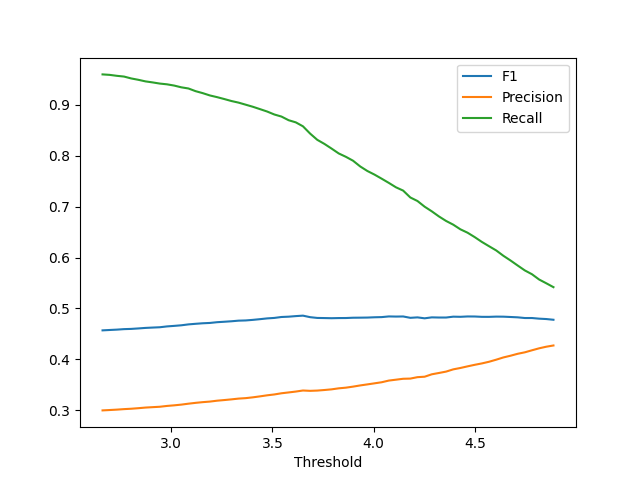
\includegraphics[width=0.7\textwidth]{TFIDF_precision_recall_f1.png}
        \label{fig:TFIDF_thresh}}
    \qquad
    \subfloat[Subfigure 2][Optimize TF-IDF threshold (3.8092) to maximize positive class (Entity = True) $F_1$ score.]{
        \begin{tabular}{lrrrr}
\toprule
             &  Precision &  Recall &  F1-Score &  Support \\
\midrule
       False &       0.88 &    0.59 &      0.71 &    38323 \\
        True &       0.24 &    0.61 &      0.34 &     8112 \\
   Macro Avg &       0.56 &    0.60 &      0.52 &    46435 \\
Weighted Avg &       0.77 &    0.59 &      0.64 &    46435 \\
\bottomrule
\end{tabular}

        \label{fig:TFIDF_classification_report}}
    \caption{Precision-Recall tradeoff curve and prediction results using TF-IDF scoring.}
    \label{fig:TFIDF}
\end{figure}

\textbf{Analysis}: The results show..

\subsubsection{TextRank to score noun phrases, threshold scores, predict entities}
Same pattern

\textbf{Analysis:} ...

\subsubsection{Use cosine similarity between encoded noun phrases and an encoded phrase such as ``this is an entity"}

This procedure..

\textbf{Analysis:} This approach..

\subsubsection{Naively predict proper nouns}
This approach...

\begin{table}[ht]
    \centering
    \begin{tabular}{lrrrr}
\toprule
             &  Precision &  Recall &  F1-Score &  Support \\
\midrule
       False &       0.98 &    0.95 &      0.96 &    38323 \\
        True &       0.78 &    0.90 &      0.84 &     8112 \\
   Macro Avg &       0.88 &    0.92 &      0.90 &    46435 \\
Weighted Avg &       0.94 &    0.94 &      0.94 &    46435 \\
\bottomrule
\end{tabular}

    \caption{Entity detection prediction results using noun phrases.}
    \label{tab:NNP}
\end{table}

\textbf{Analysis:} The results show...

\subsubsection{Use a pre-trained entity detector}
We attempt...

\textbf{Analysis:} The results...

\subsubsection{Other directions}

Here are some other things worth trying.

\section{Conclusions and future work}

It would be valuable to evaluate these methods against the ACE dataset \cite{ACE} and OntoNotes 5.0 dataset \cite{OntoNotes}.

...

The next set of logical experiments that work with entities are:
\begin{enumerate}
    \item first idea
          \begin{enumerate}
              \item sub component
              \item sub component
          \end{enumerate}
    \item second idea
\end{enumerate}

Closing remarks.

\clearpage

\printbibliography

\end{document}